\section{Appendice}

\subsection{Spettri a vari angoli}\label{appendice_spettri}
\begin{figure}[htbp]
    \centering
    % First row
    \begin{subfigure}[b]{0.45\textwidth}
        \centering
        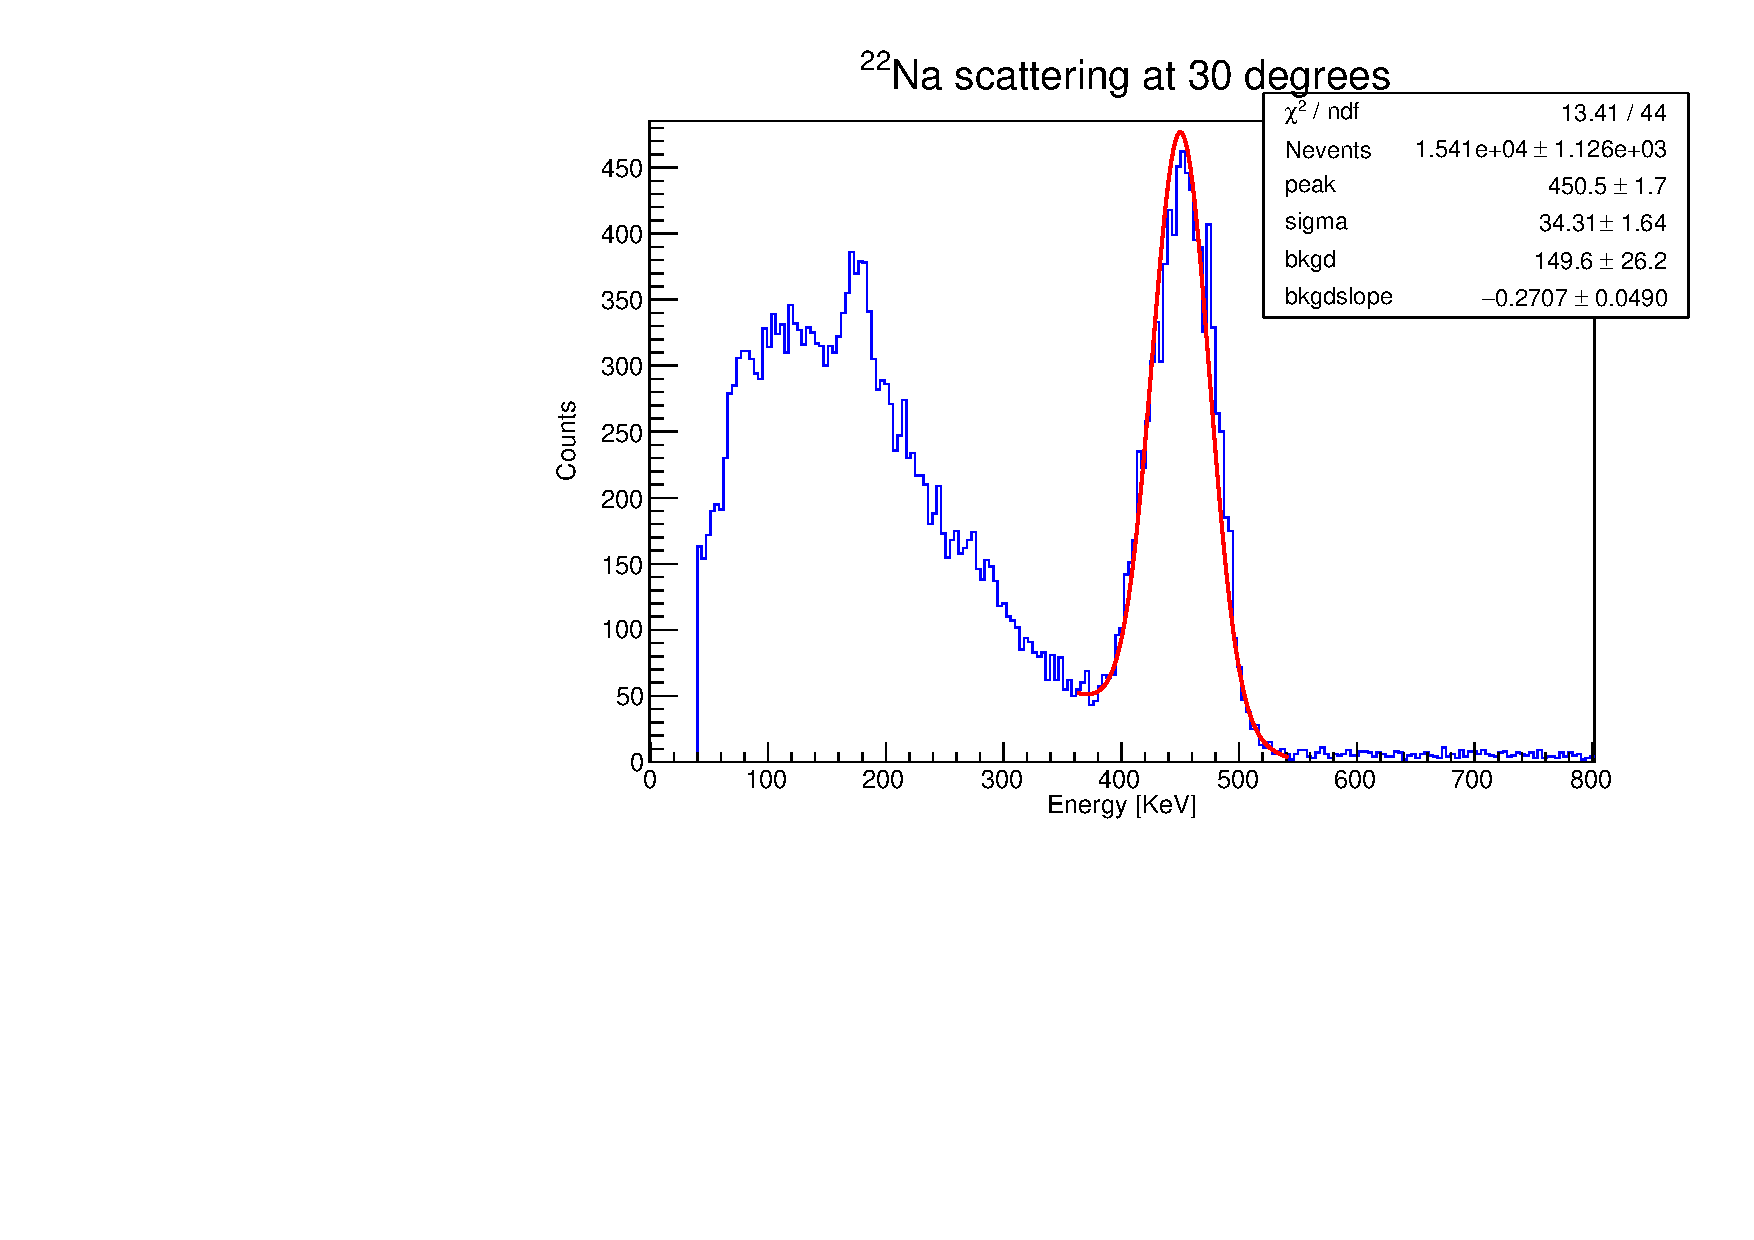
\includegraphics[width=\textwidth]{Appendice/30_deg_spectrum.pdf}
    \end{subfigure}
    \hfill
    \begin{subfigure}[b]{0.45\textwidth}
        \centering
        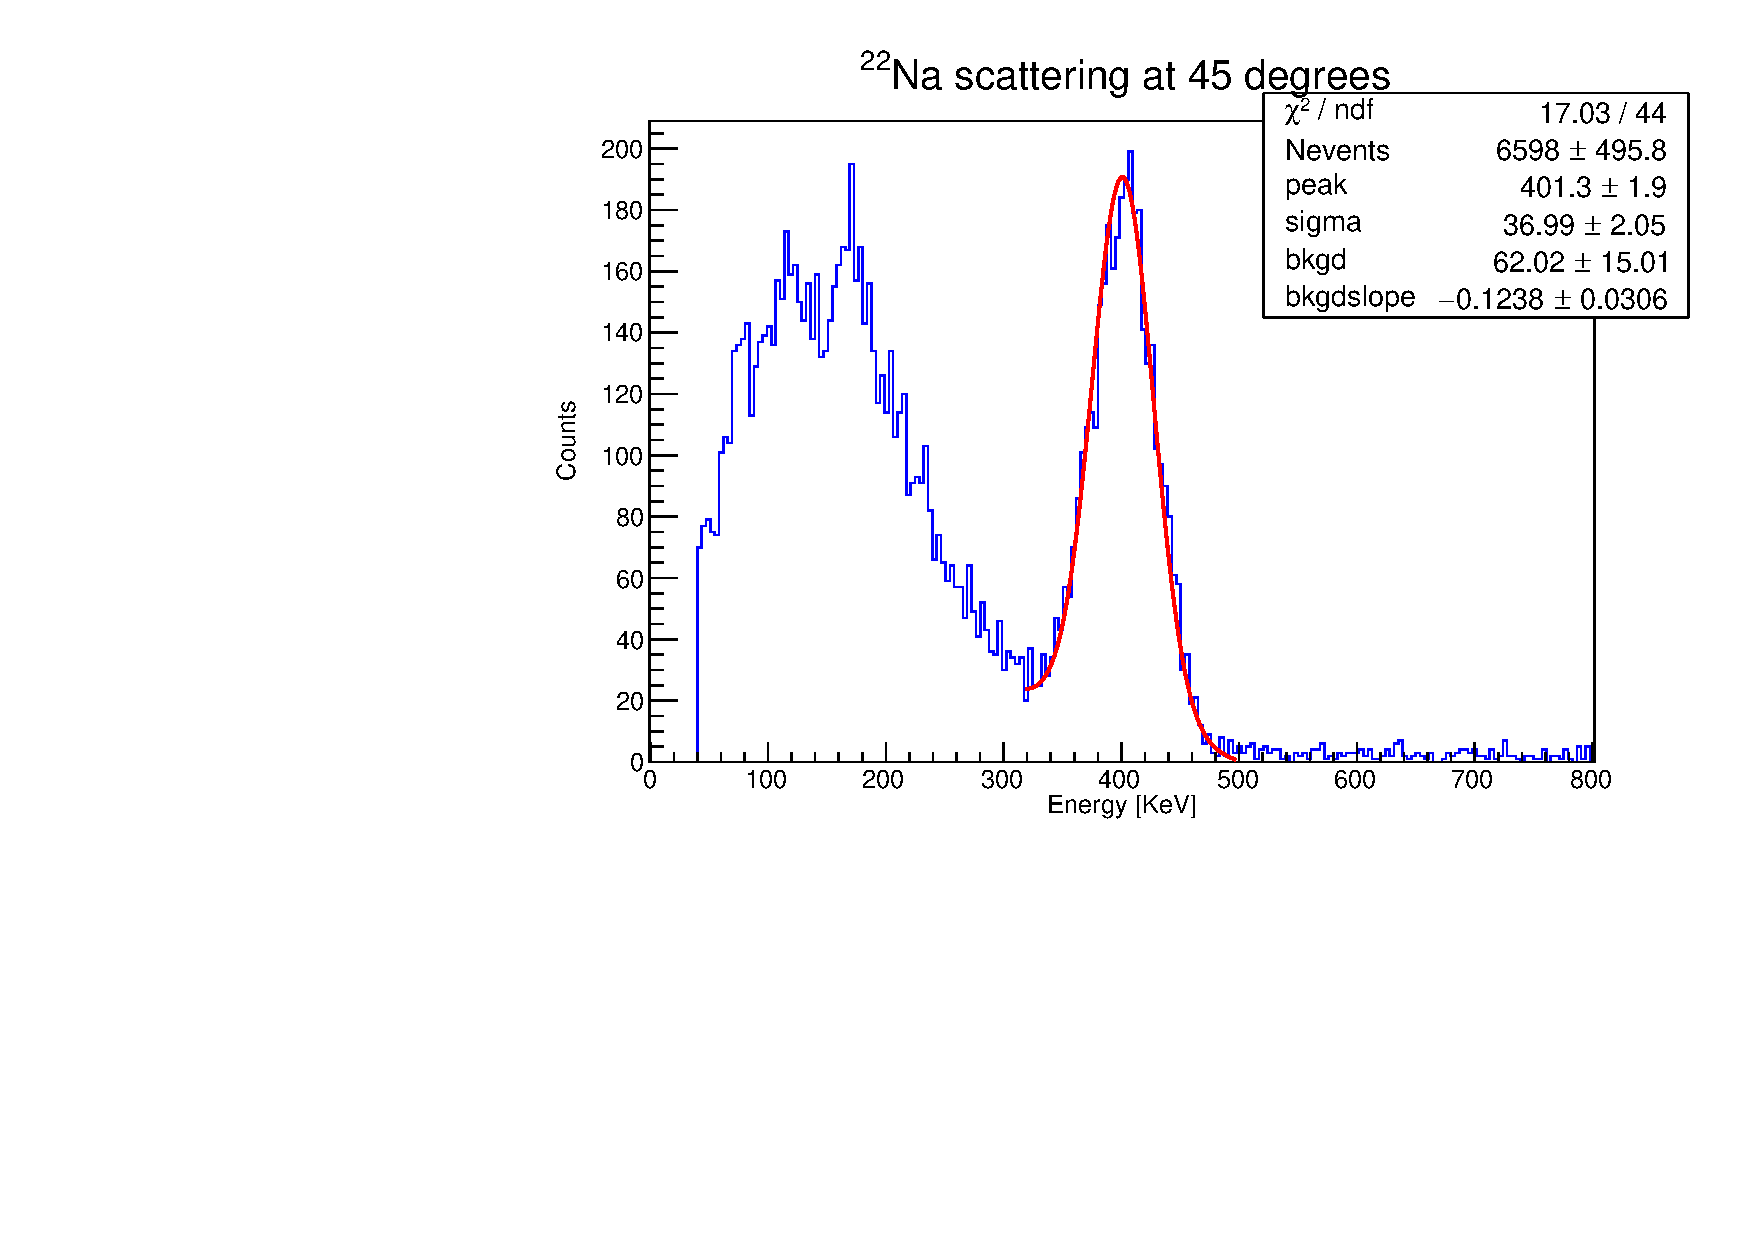
\includegraphics[width=\textwidth]{Appendice/45_deg_spectrum.pdf}
    \end{subfigure}
    
    \vspace{0.5cm} % Add vertical space between rows

    % Second row
    \begin{subfigure}[b]{0.45\textwidth}
        \centering
        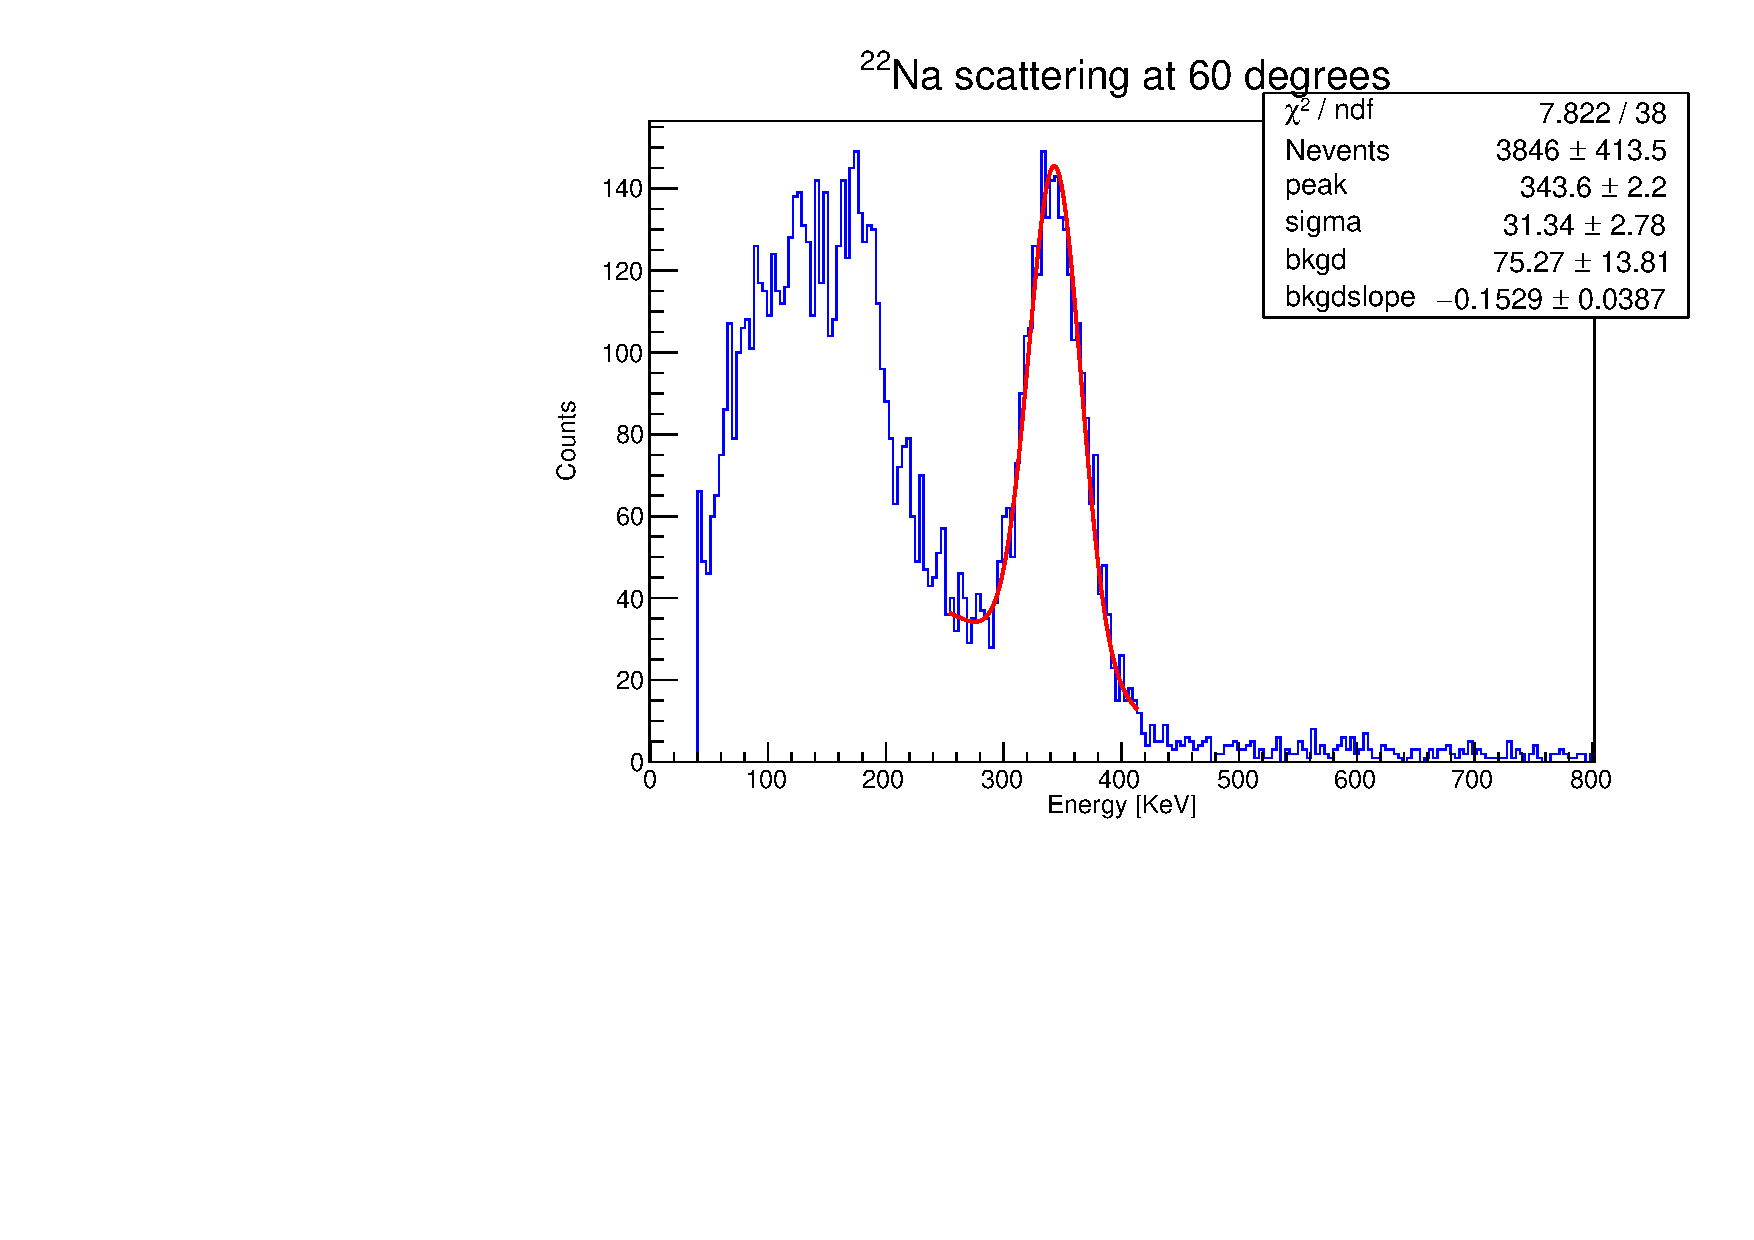
\includegraphics[width=\textwidth]{Appendice/60_deg_spectrum.pdf}
    \end{subfigure}
    \hfill
    \begin{subfigure}[b]{0.45\textwidth}
        \centering
        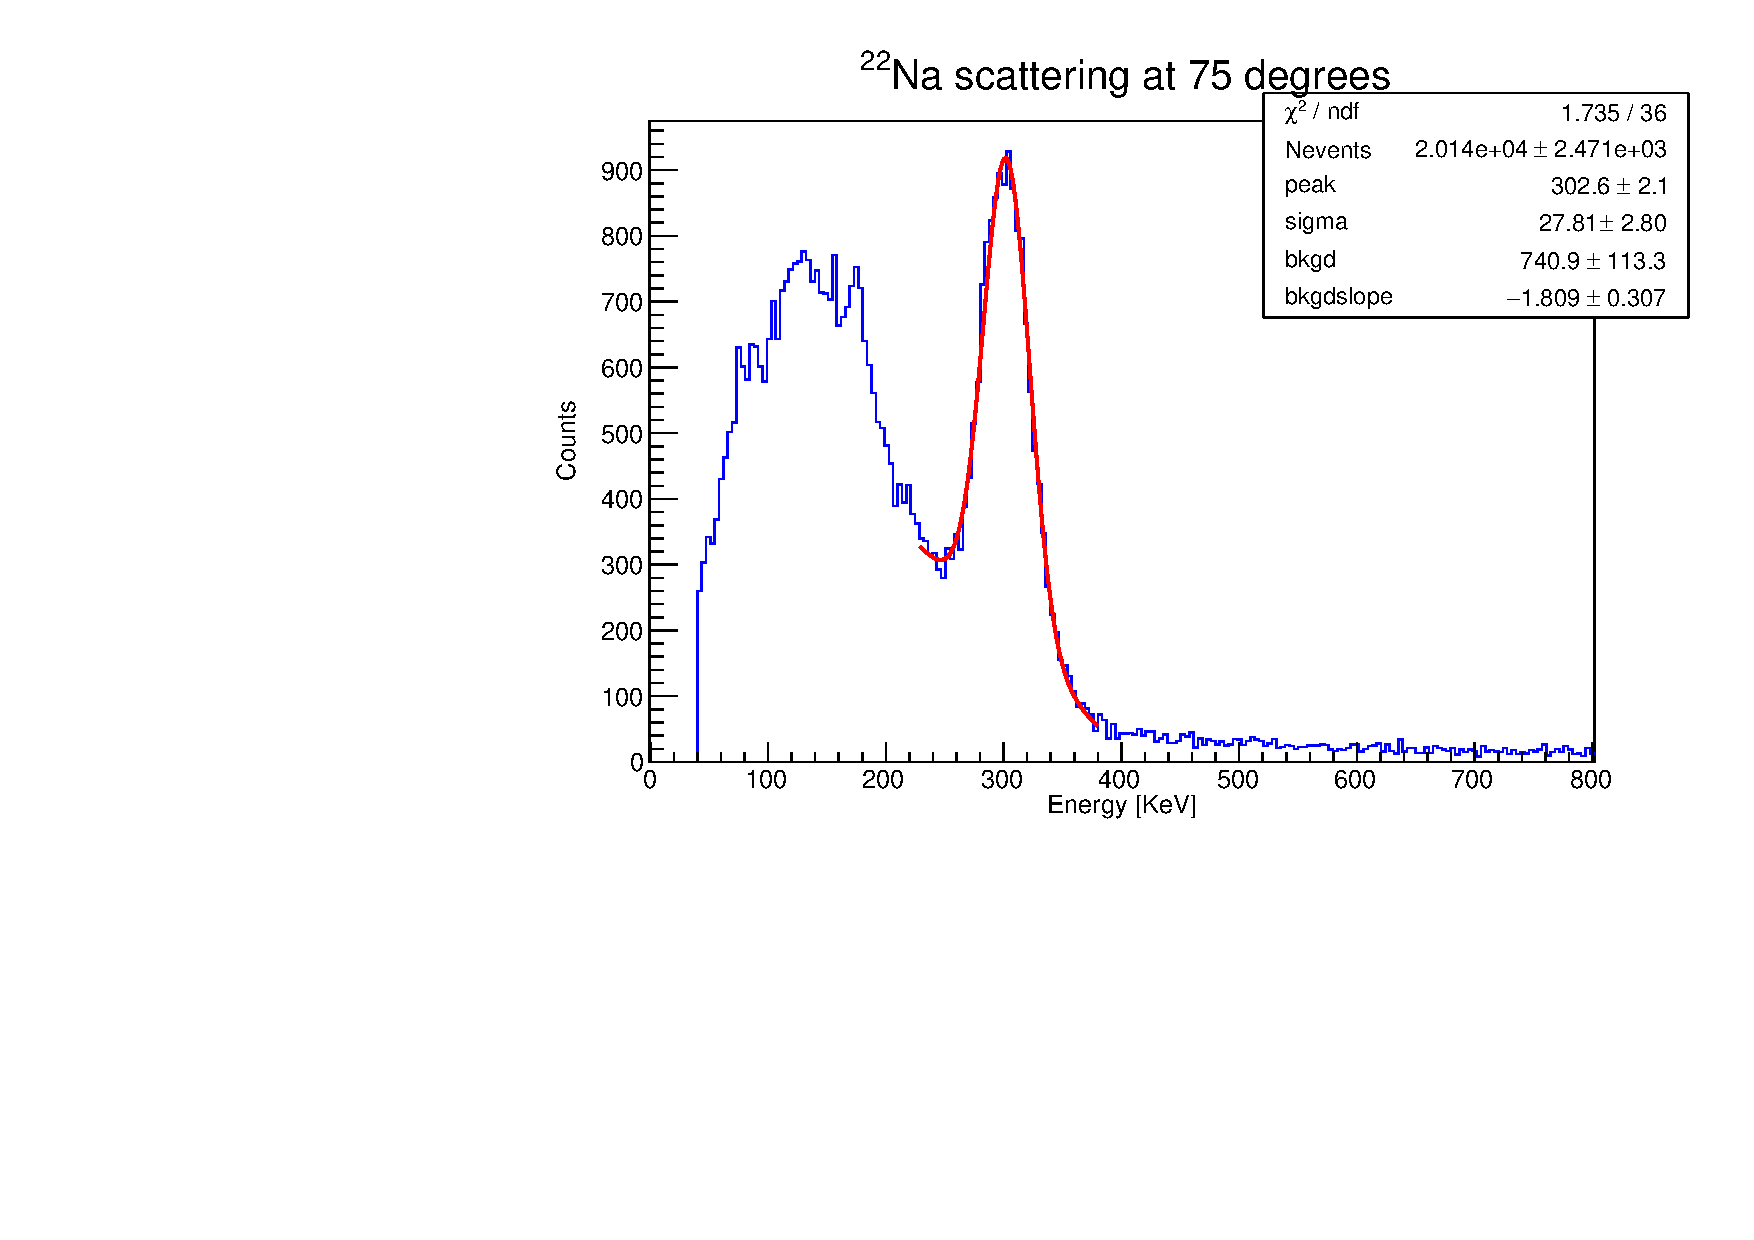
\includegraphics[width=\textwidth]{Appendice/75_deg_spectrum.pdf}
    \end{subfigure}
    
    \vspace{0.5cm} % Add vertical space between rows

    % Third row
    \begin{subfigure}[b]{0.45\textwidth}
        \centering
        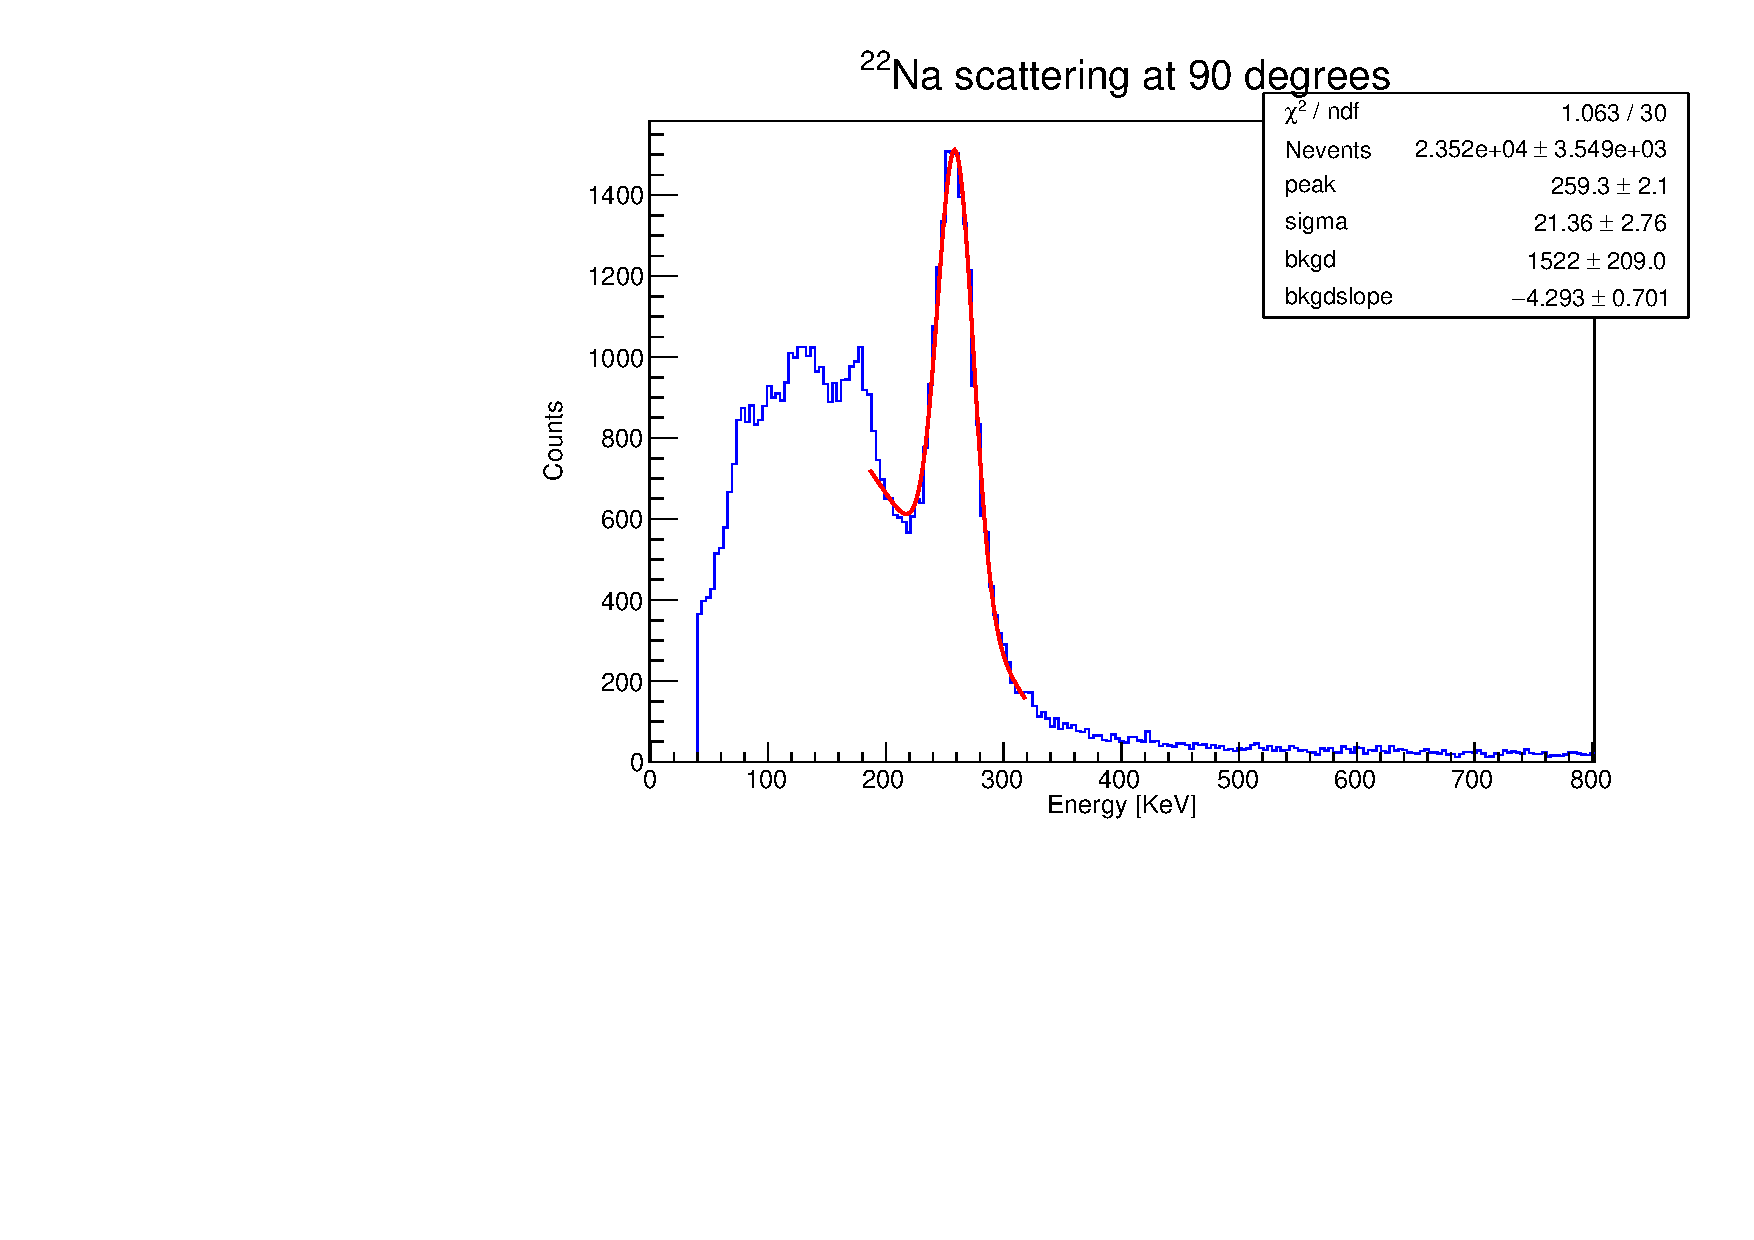
\includegraphics[width=\textwidth]{Appendice/90_deg_spectrum.pdf}
    \end{subfigure}
    \hfill
    \begin{subfigure}[b]{0.45\textwidth}
        \centering
        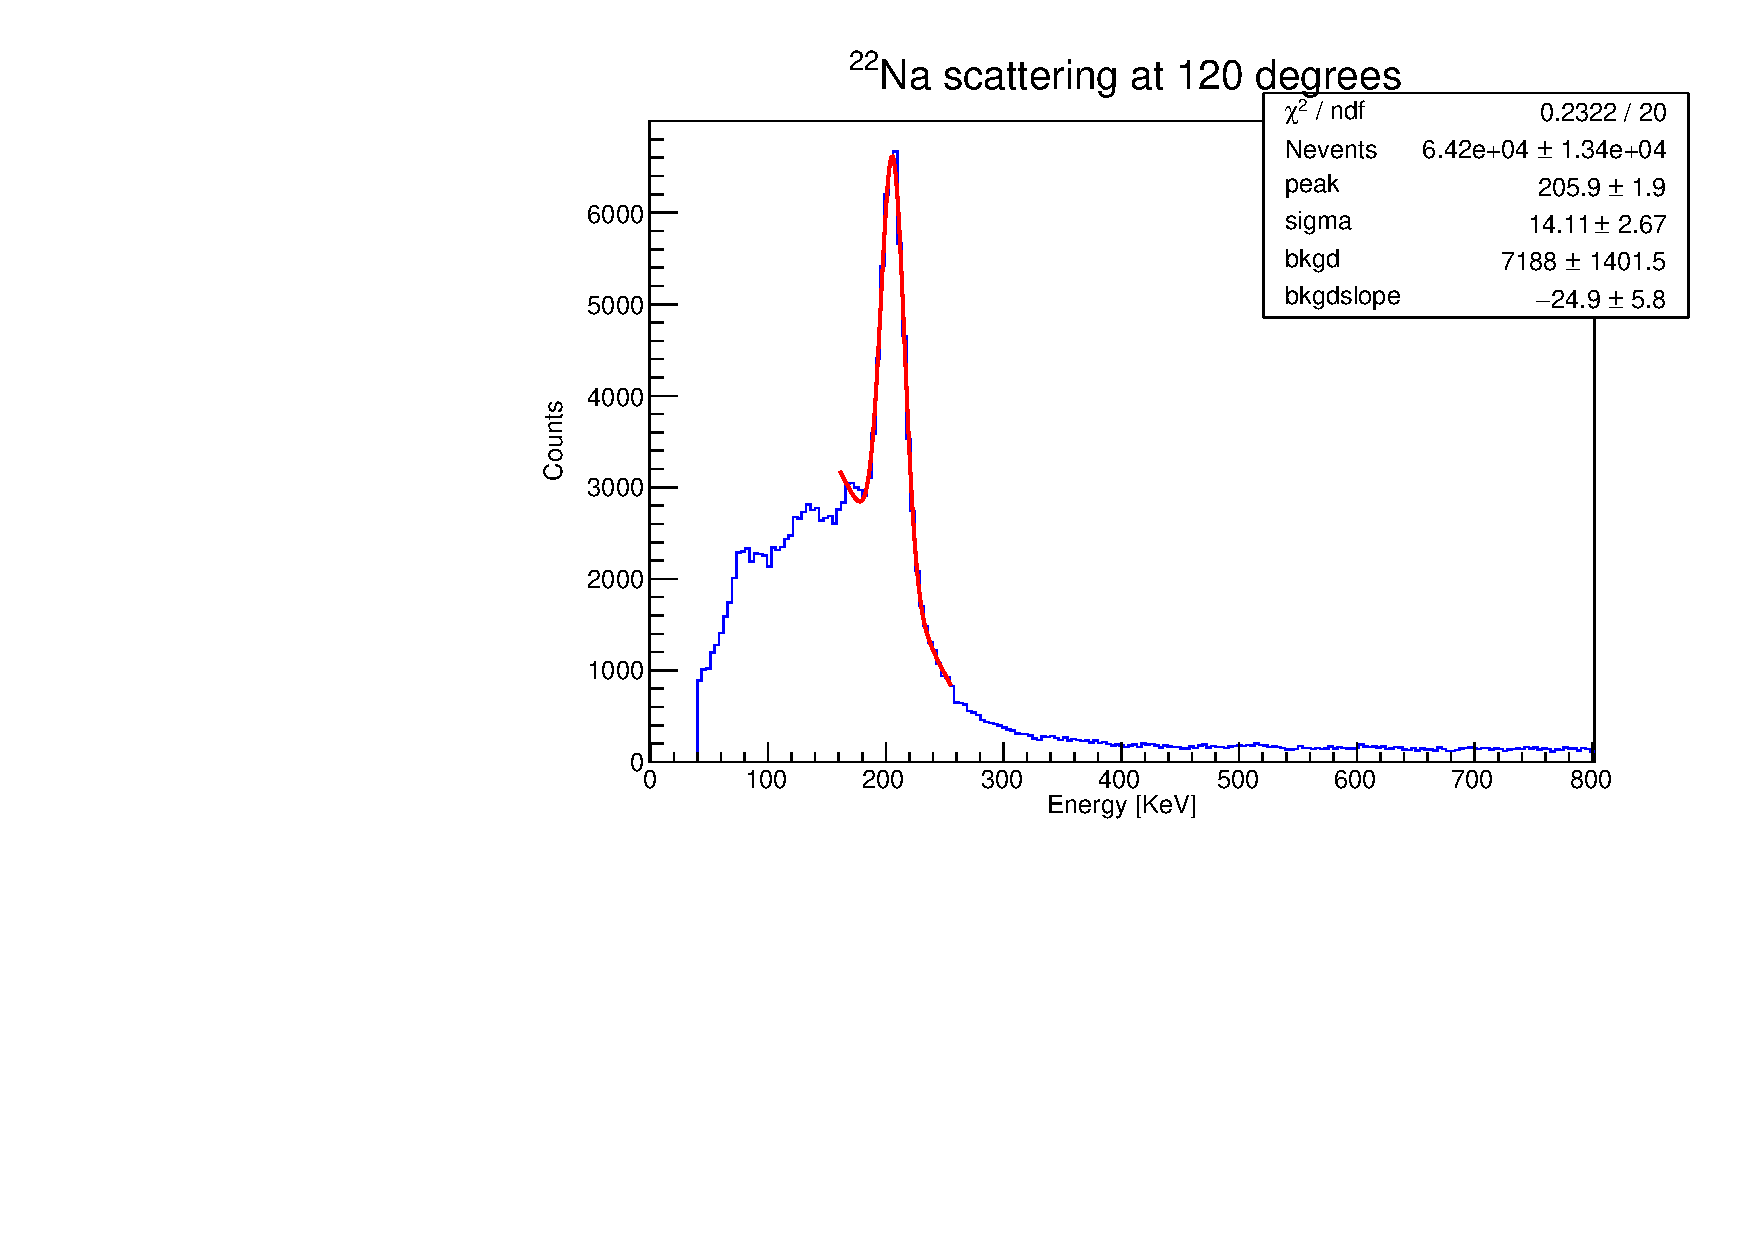
\includegraphics[width=\textwidth]{Appendice/120_deg_spectrum.pdf}
    \end{subfigure}
    
    \caption{Spettri acquisiti ai vari angoli}
    \label{fig:appendice_spettri}
\end{figure}

%\subsection{Errore sezione d'urto energetica}\label{appendice_errore_sezione_energie}
%L'errore calcolato per progazione della formula di Klein-Nishina risulta il seguente:
%\begin{equation}
   % \sigma_{\frac{d\sigma}{d\theta}} = r_e^2 \sqrt{\left( \frac{9}{4} k_1 + \frac{1}{4} + k_1^2\sin{\theta}^4+\frac{3}{2} k_1^2 -3k_1^3 \sin{\theta}^2-k_1\sin{\theta}^2 \right)\sigma_{k_1}^2 + \left(k_1^4 \sin{\theta}^2 \cos{\theta}^2\right) \sigma_{\theta}^2}
    \label{err_klein_nishina}
%\end{equation}
%dove $k_1 = \frac{E_1}{m_e c^2}$
\subsection{Dati grezzi}
\begin{table}[H]
    \centering
    \begin{tabular}{|c|c|c|c|c|}
    \hline
       Sorgente & $E_{teorica} [\unit{\kilo\electronvolt}]$ & $\sigma_{teorica}$ & ADC Channel & $\sigma_{ch}$\\
       \hline
       \hline
       $\ch{^{22}Na}$ & $511.000$ & $0.001$ & $1374.00$ & $45.87$\\
        \hline
       $\ch{^{22}Ne}$ & $1274.537$ & $0.01$ & $3439.23$ & $56.42$\\
       \hline
       $\ch{^{137}Cs}$ & $661.657$ & $0.003$ & $1783.36$ & $52.02$\\
       \hline
    \end{tabular}
    \caption{Misure dagli spettri di calibrazione ADC.}
    \label{tab:ADC}
\end{table}
\begin{table}[H]
    \centering
    \begin{tabular}{|c|c|c|c|c|c|}
    \hline
       Angolo & $E_{teorica} [\unit{\kilo\electronvolt}]$ & $E_{misurata}[\unit{\kilo\electronvolt}]$ & $\sigma$ & $N_{picco}$ & $\sigma/\sqrt{N}$\\
       \hline
       \hline
       $0^\circ$ & $511.000$ & $507.831$ & $15.97$ & $23800$ & $0.104$ \\
        \hline
       $30^\circ$ & $450.627$ & $450.451$ & $34.31$ & $8919$ & $0.363$ \\
       \hline
       $45^\circ$ & $395.238$ & $401.287$ & $36.99$ & $3790$ & $0.601$ \\
       \hline
       $60^\circ$ & $340.667$ & $343.667$ & $31.34$ & $3002$ & $0.572$ \\
       \hline
       $75^\circ$ & $293.479$ & $302.629$ & $27.81$ & $17986$ & $0.207$ \\
       \hline
       $90^\circ$ & $255.500$ & $259.277$ & $21.37$ & $27831$ & $0.128$ \\
       \hline
       $120^\circ$ & $204.400$ & $205.918$ & $14.11$ & $84629$ & $0.048$ \\
       \hline
    \end{tabular}
    \caption{Misure dagli spettri ai vari angoli.}
    \label{tab:appendice_spettri}
\end{table}
\begin{table}[H]
    \centering
    \begin{tabular}{|c|c|c|c|c|}
    \hline
       angoli& $N_i$ & $N_S$ & $\frac{N_s}{N_i}$ & $\sigma_{\frac{N_s}{N_i}}$\\
       \hline
       \hline
       $30^\circ$ & $7500140$ & $28398$ & $0.00379$ & $0.00002$\\
        \hline
       $45^\circ$ & $3882437$ & $11786$ & $0.00304$ & $0.00003$\\
       \hline
       $60^\circ$ & $3590958$ & $8661$ & $0.00241$ & $0.00003$\\
       \hline
       $90^\circ$ & $7676854$ & $14245$ & $0.00186$ & $0.00002$\\
       \hline
    \end{tabular}
    \caption{In questa tabella sono riportati i dati ricavati dalle misure in laboratorio.}
    \label{tabella dati}
\end{table}
\begin{table}[H]
    \centering
    \begin{tabular}{|c|c|c|c|}
    \hline
       $\Delta \Omega\,[\unit{sr}]$& $\sigma_{\Delta \Omega}\,[\unit{sr}]$ & $dx\,[\unit{cm}]$ & $\sigma_{dx}\,[\unit{cm}]$ \\
       \hline
       \hline
       $0.06098$ & $0.00844$ & $2.02$ & $0.05$\\
       \hline
    \end{tabular}
    \caption{In questa tabella sono presenti i dati utilizzati per calcolare la sezione d'urto,}
    \label{tabella}
\end{table}